%%%%%%%%%%%%%%%%%%%%%%%%%%%%%%%%%
\chapter{Splitting and Extension Lemmas}\label{ch:splitting-and-extension}
This chapter develops two fundamental technical tools needed for the construction of nested sweepouts: the \emph{extension lemma} and the \emph{splitting lemma}. The extension lemma allows us to modify a nested family of hypersurfaces to accommodate a new endpoint hypersurface while controlling the area increase. The splitting lemma, based on Falconer's projection theorem, enables us to construct a nested family connecting two nested regions with controlled slice areas.

\section{The Extension Lemma}\label{sec:extension-lemma}
The extension lemma is a key ingredient in the monotonisation algorithm. It allows us to insert or remove a hypersurface at one endpoint of a nested family while keeping the area bounded.

         \begin{figure}[h]
            \centering
            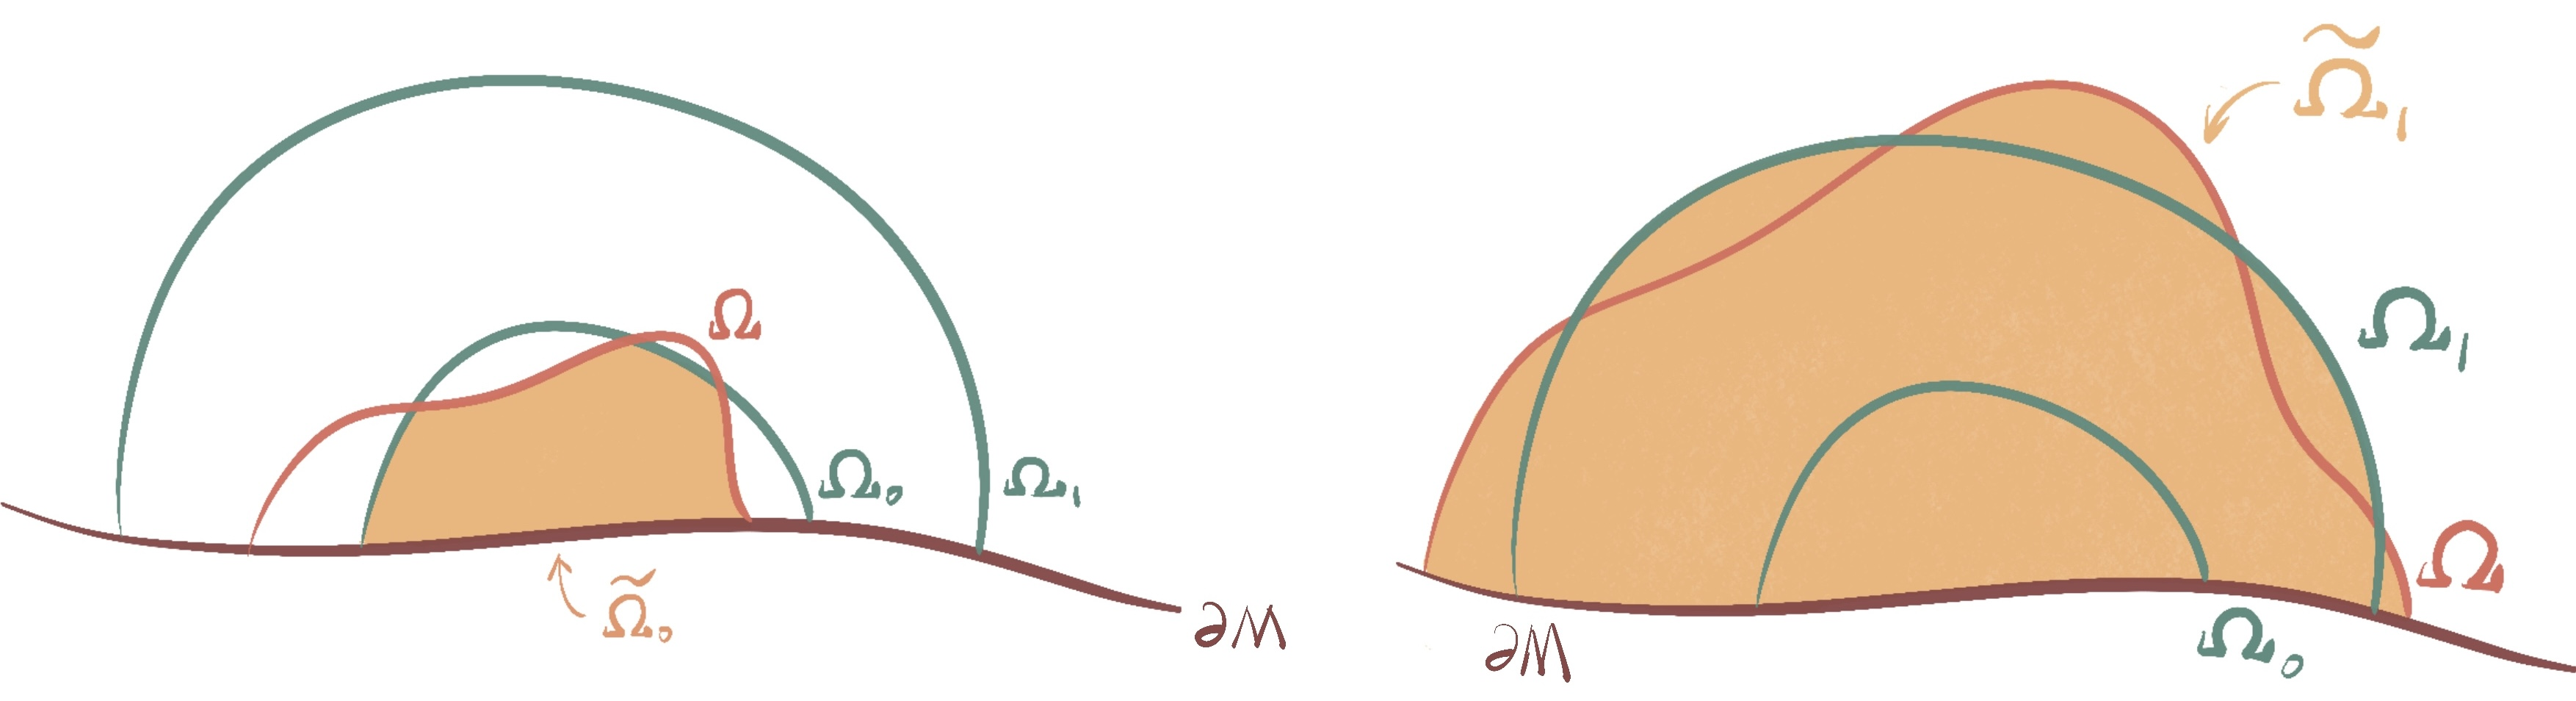
\includegraphics[width=0.8\textwidth]{figures/IMG_2674.jpg}
            \caption{Illustration of the Lemma~\ref{lem:extension} (Cases I when $\Omega \neq \Omega_0$ and II when $\Omega \neq \Omega_1$).}
            \label{fig:2674}
        \end{figure}
\begin{lemma}\label{lem:extension}
    Suppose that $f: \Tilde{M} \to [-1, \infty)$ is a Morse function and $\br{\Gamma_t} = \br{f^{-1}(t)}_{t \in [0, 1]}$ is a nested family of hypersurfaces such that $\haus^n(\Gamma_t\cap M) \leq A$ for all $t \in [0, 1]$ with associated open sets $\br{\Omega_t} = \br{f^{-1}((-\infty, t))}$.
    \begin{enumerate}
        \item[I.] Suppose $\Omega$ is a bounded open set with boundary $\Gamma$ a smooth embedded manifold such that
        \begin{enumerate}
            \item[(1)] $\Omega\subset\Omega_1$;
            \item[(2)] There is an $\eps > 0$ such that for every $\Omega'$ with $\Omega \subset \Omega'\subset \Omega_1$ we have
            \begin{equation*}
                \haus^n(\Gamma\cap M) < \haus^n(\partial_{rel}\Omega') + \frac{\eps}{4}.
            \end{equation*}
        \end{enumerate}
        Then, we can find a nested family $\br{\Tilde{\Gamma}_t}$ and an associated family of open sets $\br{\Tilde{\Omega}_t}$ such that $\Tilde{\Omega}_0 \subset \Omega_0$, $\Tilde{\Gamma}_1 = \Gamma$ and for all $t \in [0, 1]$
        \begin{equation*}
            \haus^n(\Tilde{\Gamma}_t\cap M) \leq A + \eps.
        \end{equation*}
        Furthermore, if $\Omega_0 \subset \Omega$, then $\Tilde{\Gamma}_0 = \Gamma_0$.
        \item[II.] Suppose that instead of properties (1) and (2) above, the following are true:
        \begin{enumerate}
            \item[(1)'] $\Omega_0 \subset \Omega$;
            \item[(2)'] There is an $\eps > 0$ such that for every $\Omega'$ with $\Omega_0\subset \Omega'\subset \Omega$ we have 
            \begin{equation*}
                \haus^n(\Gamma\cap M) < \haus^n(\partial_{rel}\Omega') + \frac{\eps}{4}.
            \end{equation*}
        \end{enumerate}
        Then, we can find a nested family $\br{\Tilde{\Gamma}_t}$ and an associated family of open sets $\br{\Tilde{\Omega}_t}$ such that $\Omega_1 \subset \Tilde{\Omega}_1$, $\Tilde{\Omega}_0 = \Gamma$, and for all $t \in [0, 1]$
        \begin{equation*}
            \haus^n(\Tilde{\Gamma}_t\cap M) \leq A + \eps.
        \end{equation*}
        Furthermore, if $\Omega \subset \Omega_1$, then $\Tilde{\Gamma}_1 = \Gamma_1$. 
    \end{enumerate}
    \begin{proof}
        We begin the proof with the first half of this lemma.
        The desired family will be obtained by regularization of the collection of hypersurfaces $\br{\partial(\Omega_0\cap \Omega)}$. As in the left side of Figure~\ref{fig:2674}.
        \begin{itemize}
            \item \textbf{Case I(a) $\Omega\subset \Omega_0$:}\\
            For a sufficiently small $\delta > 0$ the function $g: cl(N_{\delta}(\Gamma)\cap \Omega)\to [0, 1]$ given by $g(x) = \frac{1}{\delta}\dist(x, \Gamma)$ is a smooth function without critical points and $\Tilde{\Gamma}_t = g^{-1}(t)$ would satisfy
            \begin{equation*}
                \haus^n(\Tilde{\Gamma}_t\cap M) \leq \haus^n(\Gamma\cap M) + \frac{\eps}{2}.
            \end{equation*}
            By I(2) and $\Omega \subset \Omega_0 \subset \Omega_1$, we know that 
            \begin{equation*}
                \haus^n(\Gamma\cap M) \leq \haus^n(\partial_{rel}\Omega_0) + \frac{\eps}{4}
            \end{equation*}
            thus
            \begin{equation*}
                \haus^n(\Tilde{\Gamma}_t\cap M) \leq A + \eps.
            \end{equation*}
            We extend $g$ to a Morse function on $M$ in an arbitrary way and $\br{\Tilde{\Gamma}_t}$ is a nested family satisfying the conditions of the theorem.
            \item \textbf{Case I(b) $\Omega\backslash \Omega_0 \neq \varnothing$:}\\
            Make a small perturbation to the hypersurface $\Gamma = \partial\Omega$ so that $f|_{\partial\Omega}$ is a Morse and (1) and (2) are still satisfied, possibly replacing $\eps/4$ in (2) by $\eps/2$.

            Consider $f$ restrict to $\Omega$. We apply Lemma~\ref{lem:morse-foliation-1} with $N = \Omega$ and $\Sigma = \Gamma$ to obtain a Morse function $g: \Omega \to [-1, 1]$ for $\eps/2$ such that $g^{-1}(-1)$ is a point in $\Omega$ and 
            \begin{enumerate}
                \item $g^{-1}(1) = \Gamma$;
                \item $f^{-1}([-1, t)) \subset N_{\eps/4}(g^{-1}([-1, t))) \subset N_{\eps/2}(f^{-1}([-1, t)))$;
                \item $\haus^n(g^{-1}(t)\cap M) \leq \haus^n(\partial f^{-1}([-1, t])\cap M) + \eps/2$;
                \item If $\dist(x, f(\Gamma)) \geq \eps/2$ then $f^{-1}(x) = g^{-1}(x)$.
            \end{enumerate}
            It follows that from 3. that
            \begin{equation*}
                \begin{split}
                    \haus^n(g^{-1}(t)\cap M) \leq& \haus^n((f^{-1}(t)\cap \Omega)\cap M)\\
                    &+ \haus^n((f^{-1}([-1, t])\cap \Gamma)\cap M) + \frac{\eps}{2}
                \end{split}
            \end{equation*}
            Furthermore, we have
            \begin{equation*}
                g^{-1}([-1, 0)) \subset N_\eps(\Omega\cap \Omega_0).
            \end{equation*}
            After a small perturbation of the function $g$ we may assume that $g^{-1}([-1, 0)) \subset (\Omega\cap\Omega_0)$. We can extend $g$ to a Morse function in an arbitrary way. We claim that $\Tilde{\Gamma}_t = g^{-1}(t)$ for $t \in [0, 1]$ is the desired nested family and the only thing left is to prove the upper bound for the areas of $\Tilde{\Gamma}_t$.

            For any smooth hypersurface $\Sigma_t$ obtained by a small perturbation of $\partial(\Omega\cup\Omega_t)$ since $\Omega \subset (\Omega\cup\Omega_t) \subset \Omega_1$. It follows that 
            \begin{equation*}
                \haus^n(\Gamma\cap M) \leq \haus^n(\Sigma_t\cap M) + \frac{\eps}{4}
            \end{equation*}
            Furthermore, it follows that
            \begin{equation*}
                \haus^n(\Gamma\cap M) \leq \haus^n(\partial_{rel}(\Omega\cup\Omega_t)) + \frac{\eps}{2}
            \end{equation*}
            Since $\partial(\Omega\cup\Omega_t) = (\Gamma_t\backslash\Omega)\cup(\Gamma\backslash\Omega_t)$ we have
            \begin{equation*}
                \begin{split}
                    &\haus^n((\Gamma\cap\Omega_t)\cap M) + \haus^n((\Gamma\backslash\Omega_t)\cap M) \\
                    &\leq \haus^n((\Gamma_t\backslash\Omega)\cap M) + \haus^n((\Gamma\backslash\Omega_t)\cap M) + \eps/2\\
                    \implies & \haus^n((\Gamma\cap\Omega_t)\cap M) \leq \haus^n((\Gamma_t\backslash\Omega)\cap M) + \eps/2
                \end{split}
            \end{equation*}
        By Lemma~\ref{lem:morse-foliation-1}, we have
        \begin{equation*}
            \begin{split}
                \haus^n(\Tilde{\Gamma}_t\cap M) \leq& \haus^n((\Gamma_t\cap \Omega)\cap M) + \haus^n((\Gamma\cap\Omega_t)\cap M) + \frac{\eps}{2}\\
                \leq& \haus^n((\Gamma_t\cap \Omega)\cap M) + \haus^n((\Gamma_t\backslash\Omega)\cap M) + \eps\\
                \leq& \haus^n(\Gamma_t\cap M) + \eps \leq A + \eps
            \end{split}
        \end{equation*}
        \end{itemize}
        If $\Omega_0 \subset \Omega$, then by choosing sufficiently small $\eps > 0$ and applying Lemma~\ref{lem:morse-foliation-1}(4), we have
        \begin{equation*}
            \Tilde{\Gamma}_0 = f^{-1}(0) = \Gamma_0.
        \end{equation*}
        The proof of the second half is similar. The desired family will be a regularization of $\br{\partial(\Omega_t\cup \Omega)}$.
        \begin{itemize}
            \item \textbf{Case II(a) $\Omega_1 \subset \Omega$:}\\
            We define the desired nested family $\br{\Tilde{\Gamma}_t}$ in a small tubular neighbourhood of $\Gamma$.
            \item \textbf{Case II(b) $\Omega_1\backslash\Omega \neq \varnothing$:}
            We define $\Tilde{f}(x) = -f(x)$. We apply Lemma~\ref{lem:morse-foliation-non-compact} to $N = \Tilde{M}\backslash\Omega$ and $\Sigma = \Gamma$ and the restriction $\Tilde{f}: \Tilde{M}\backslash\Omega \to (-\infty, 0]$. It follows that given $\eps/2$, there exists a Morse function
            $\Tilde{g}: \Tilde{M}\backslash\Omega \to (-\infty, 0]$, such that 
            \begin{enumerate}
                \item $\Tilde{g}^{-1}(0) = \Gamma$;
                \item $\Tilde{f}^{-1}((-\infty, t)) \subset N_{\eps/4}(\Tilde{g}^{-1}((-\infty, t))) \subset N_{\eps/2}(\Tilde{f}^{-1}((-\infty, t)))$;
                \item $\haus^n(\Tilde{g}^{-1}(t)\cap M) \leq \haus^n(\partial\Tilde{f}^{-1}((-\infty, t])\cap M) + \frac{\eps}{2}$;
                \item If $\dist(x, \Tilde{f}(\Sigma)) > \eps$ then $\Tilde{f}^{-1}(x) = \Tilde{g}^{-1}(x)$.
            \end{enumerate}
            We define $g(x) = -\Tilde{g}(x)$ for $x \in \Tilde{M}\backslash\Omega$ and extend it to a Morse function from $\Tilde{M}$ to $[-1, \infty)$ in an arbitrary way. By property (2) of Lemma~\ref{lem:morse-foliation-non-compact} we take that (possibly after a small perturbation)
            \begin{equation*}
               \Tilde{\Omega}_1 := g^{-1}([-1, 1]) \supset \Omega_1
            \end{equation*}
            For any smooth hypersurface $\Sigma_t$ obtained by a small perturbation of $\partial(\Omega\cap\Omega_t)$. By (2)', we have
            \begin{equation*}
                \haus^n(\Gamma\cap M) \leq \haus^n(\Sigma_t\cap M) + \frac{\eps}{4} 
            \end{equation*}
            Furthermore, it follows that
            \begin{equation*}
                \haus^n(\Gamma\cap M) \leq \haus^n(\partial_{rel}(\Omega\cap\Omega_t)) + \frac{\eps}{2}
            \end{equation*}
            Since $\partial(\Omega\cap \Omega_t) = (\Gamma_t\cap\Omega)\cup(\Gamma\cap\Omega_t)$ we have
            \begin{equation*}
                \begin{split}
                    &\haus^n((\Gamma\cap\Omega_t)\cap M) + \haus^n((\Gamma\backslash\Omega_t)\cap M) \\
                    &\leq \haus^n((\Gamma_t\cap\Omega)\cap M) + \haus^n((\Gamma\cap\Omega_t)\cap M) + \eps/2\\
                    \implies & \haus^n((\Gamma\backslash\Omega_t)\cap M) \leq \haus^n((\Gamma_t\cap\Omega)\cap M) + \eps/2
                \end{split}
            \end{equation*}
            By Lemma~\ref{lem:morse-foliation-non-compact}, we have
        \begin{equation*}
            \begin{split}
                \haus^n(\Tilde{\Gamma}_t\cap M) \leq& \haus^n((\Gamma_t\backslash \Omega)\cap M) + \haus^n((\Gamma\backslash\Omega_t)\cap M) + \frac{\eps}{2}\\
                \leq& \haus^n((\Gamma_t\backslash \Omega)\cap M) + \haus^n((\Gamma_t\cap\Omega)\cap M) + \eps\\
                \leq& \haus^n(\Gamma_t\cap M) + \eps \leq A + \eps
            \end{split}
        \end{equation*}
        \end{itemize}
        If $\Omega \subset \Omega_1$ then by property (4) of Lemma~\ref{lem:morse-foliation-non-compact} we may assume that $\Tilde{\Gamma}_1 = g^{-1}(1) = \Gamma_1$.
    \end{proof}
\end{lemma}

\section{The Splitting Lemma}\label{sec:splitting-lemma}

The second lemma in this chapter deals with constructing a nested family between two nested open sets.

\begin{theorem}[Falconer]\label{thm:falconer}
    There exists a constant $C(n)$ so that the following is true. Let $U \subset \R^{n + 1}$ be an open set with smooth boundary. There exists a line $l \in \R^{n + 1}$ so that the projection $p_l$ onto $l$ satisfies 
    \begin{equation*}
        \vol_n(U\cap p^{-1}_l(t)) < C(n)\vol_{n + 1}(U)^{\frac{n}{n + 1}}
    \end{equation*}
    for all $t \in l$. Moreover, we can assume that $p_l$ restricted to $\partial U$ is a Morse function. 
\end{theorem}
\begin{lemma}\label{lem:existence-nested-between-sets}
    Let $\eps > 0$, $L > 0$. Suppose $\Omega_0 \subset \Omega_1$ be bounded open sets with smooth boundary and $\Omega_1 \backslash \Omega_0 \subset B$ where $B$ is $(1 + L)$-bilipschitz diffeomorphic to an relative open subset $U$ of $\R^{n + 1}_+$. There exists a constant $C(n)$ and a nested family $\br{\Gamma_t'}$ with a family of corresponding open sets $\br{\Omega_t'}$, such that
    \begin{enumerate}
        \item[(1)] the area of the new sweepout can be estimated as 
        \begin{equation*}
            \begin{split}
                \haus^n(\Gamma_t'\cap M) \leq& \haus^n(\partial\Omega_0\cap M) + \haus^n(\partial(\Omega_1\backslash\Omega_0)\cap M)\\
                &+ C(n)(1 + L)^n\haus^{n + 1}(\Omega_1\backslash\Omega_0)^{\frac{n}{n + 1}} + \eps;
            \end{split}
        \end{equation*}
        \item[(2)] $\Omega_0'$ is an relative inward $\eps$-perturbation of $\Omega_0$ and $\Omega_1' = \Omega_1$;
        \item[(2')] $\Omega_1'$ is an relative outward $\eps$-perturbation of $\Omega_1$ and $\Omega_0' = \Omega_0$;
    \end{enumerate}
    \begin{proof}
        Let $\Omega'$ be an relative inward  $\eps/8$-perturbation of $\Omega = \Omega_1\backslash\Omega_0$. By definition that means
        \begin{enumerate}
            \item[(a)] $\Omega\backslash N_\frac{\eps}{8}(\partial\Omega) \subset \Omega' \subsetneq \Omega$;
            \item[(b)] There exists a nested family of open sets $\br{\Xi_t}_{t \in [0, 1]}$ and a smooth isotopy $\Sigma_t = \partial\Xi_t$, such that $\Sigma_0$ is a smoothing of $\partial\Omega$ and $\Xi_1 = \Omega'$ such that 
            \begin{equation*}
                \haus^n(\Sigma_t\cap M) \leq \haus^n(\partial\Omega \cap M) + \frac{\eps}{8}
            \end{equation*}
            for all $t \in [0, 1]$. 
        \end{enumerate}
        By Theorem~\ref{thm:falconer}, there exists a Morse function $f: \Omega' \to [0, 1]$ such that
        \begin{equation*}
        \begin{split}
            \haus^n(f^{-1}(t)) \leq C(n)(1 + L)^n\haus^{n+1}(\Omega_1\backslash\Omega_0)^{\frac{n}{n + 1}} + \eps/4. 
        \end{split}
        \end{equation*}

        We denote the nested sweepout of $\Omega'$ from $g$ as $\br{\Sigma_t^a}$ with the corresponding family of open sets $\br{\Xi_t^a}$, such that $\Omega' = \Xi_1^a$. By Lemma~\ref{lem:morse-foliation-1}, given $\eps/4 > 0$, we can find $g: \Omega' \to [0, 1]$ such that 
        \begin{equation}\label{eq:sigma-a-t}
            \begin{split}
                \haus^n(\Sigma_t^a\cap M) &\leq \haus^n(\partial f^{-1}([0, t])\cap M) + \eps/4\\
                &\leq \haus^n(\partial(\Omega_1\backslash\Omega_0)\cap M) + C(n)(1 + L)^n\haus^{n+1}(\Omega_1\backslash\Omega_0)^{\frac{n}{n + 1}} + \eps/2.  
            \end{split}
        \end{equation}
        Let $\br{\Sigma_t^b}$ be a nested family with a corresponding family of open sets $\br{\Xi_t^b}$, such that $\br{\Xi_0^b}$ is a relative inward $\eps/2$-perturbation of $\Omega_0$, $\Xi_1^b$ is a relative inward $\eps/8$-perturbation of $\Omega_0$. For all $t \in [0, 1]$, the relative area of the slices would satisfy
        \begin{equation}\label{eq:sigma-b-t}
            \haus^n(\Sigma_t^b\cap M) \leq \haus^n(\partial\Omega_0\cap M) + \eps/2.
        \end{equation}

        By Lemma~\ref{lem:morse-separate}, there exists a nested family $\br{\Sigma_t^c}$ with the corresponding family of open sets $\br{\Xi_t^c}$, such that $\Xi_1^c = \Omega_1$, $\Xi_0^c = \Xi^1\sqcup \Xi^2$, where $\Xi^1$ is an relative inward $\eps/8$-perturbation of $\Omega_0$ and $\Xi^2$ is an relative inward $\eps/8$-perturbation of $\Omega_1\backslash\Omega_0$. It follows from the properties of the perturbations that, without any loss of generality, we may assume $\Xi^1 = \Xi_1^b$ and $\Xi^2 = \Omega'$. By (3) of Lemma~\ref{lem:morse-separate}, we have
        \begin{equation*}
        \begin{split}
            \haus^n(\Sigma_t^c\cap M) \leq& \haus^n(\partial\Omega_1\cap M) + 2\haus^n((\partial\Omega_0\backslash\partial\Omega_1)\cap M) + \eps\\
            \leq& \haus^n(\partial(\Omega_1\backslash\Omega_0)\cap M) + \haus^n(\partial\Omega_0\cap M) + \eps
        \end{split}
        \end{equation*}
        We define $\Gamma_t' = \Sigma_{2t}^a\cup\Sigma_{2t}^b$ for $t \in [0, 1/2)$ and $\Gamma_t' = \Sigma_{2t - 1}^c$, $t \in [1/2, 1]$ with the open sets defined correspondingly. Then for $t \in [0, 1/2)$ combining \ref{eq:sigma-a-t} and \ref{eq:sigma-b-t}, we obtain
        \begin{equation*}
            \begin{split}
                \haus^n(\Gamma_t'\cap M) \leq& 
                \haus^n(\Sigma_{2t}^a\cap M) + \haus^n(\Sigma_{2t}^b\cap M)\\
                \leq&  \haus^n(\partial\Omega_0\cap M) + \haus^n(\partial(\Omega_1\backslash\Omega_0)\cap M)\\
                &+ C(n)(1 + L)^n\haus^n(\Omega_1\backslash\Omega_0)^{\frac{n}{n + 1}} + \eps
            \end{split}
        \end{equation*}
    \end{proof}
\end{lemma}